
\section{Expérimentations}

\begin{figure*}
  \centering
  \subfloat[Figure A][Clustering coefficient of \CYCLON.]{
    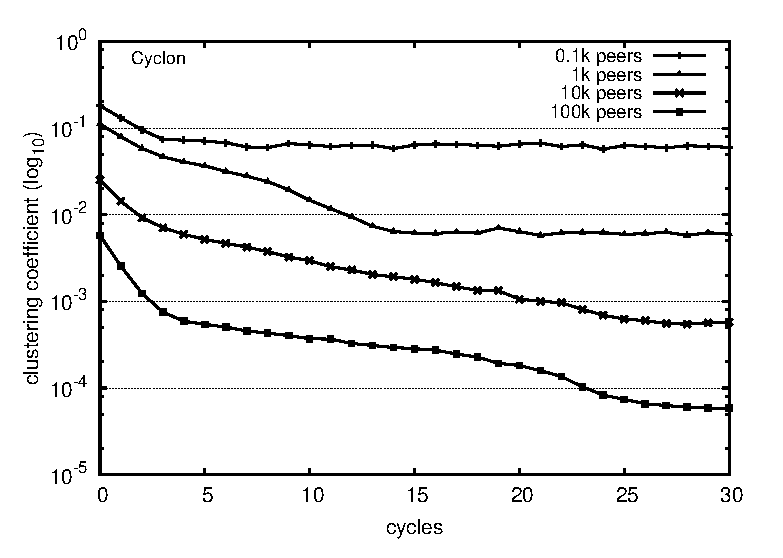
\includegraphics[width=0.47\textwidth]{img/spray/cycloncluster.eps}}
  \hspace{10pt}
  \subfloat[Figure B][Clustering coefficient of \SPRAY.]{
    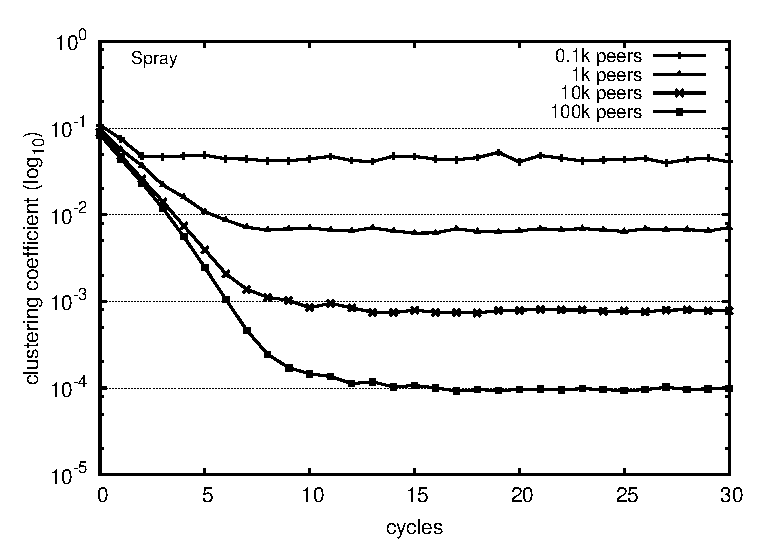
\includegraphics[width=0.47\textwidth]{img/spray/spraycluster.eps}}
  \caption{\label{fig:clustering}The x-axis denotes the elapsed time in cycles
    while the y-axis denotes the $\log_{10}$-scaled clustering coefficient.}
\end{figure*}

\begin{figure}
  \centering
  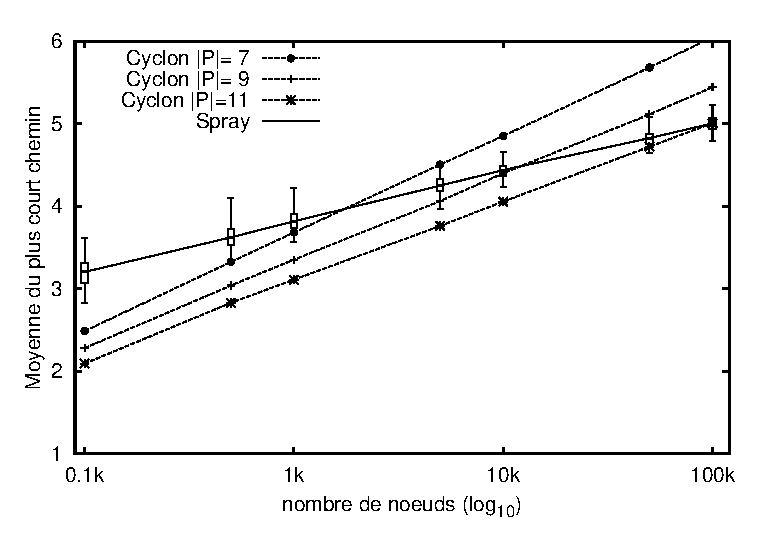
\includegraphics[width=\textwidth]{img/spray/avgpath.eps}
  \caption{\label{fig:avgpath}The average shortest path length of \SPRAY and
    \CYCLON. The x-axis denotes the number of peers in the network on a
    $\log_{10}$ scale (from 100 to 100k peers) while the y-axis denotes the
    average shortest path length of the network.}
\end{figure}

\begin{figure}
  \centering
  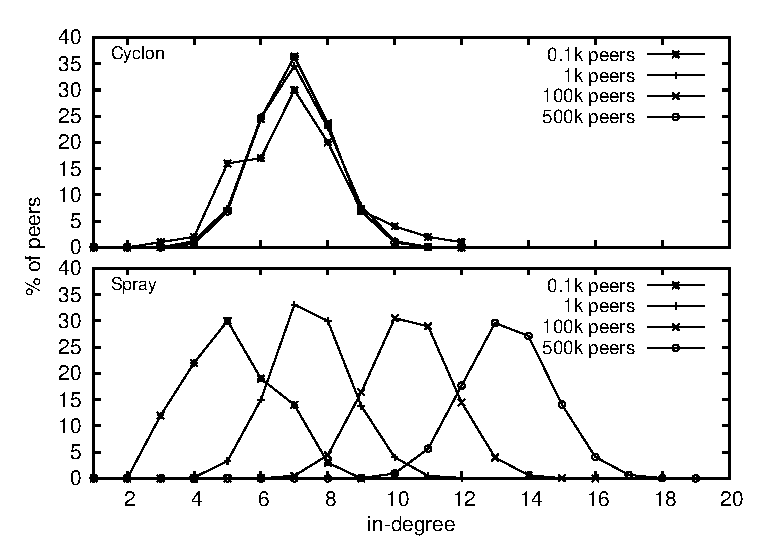
\includegraphics[width=\textwidth]{img/spray/histo.eps}
  \caption{\label{fig:histo}The in-degree distribution of \CYCLON and
    \SPRAY. The x-axis denotes the in-degree in number of nodes while the
    y-axis indicates the percentage of peers with such in-degree. The top
    figure is dedicated to the runs concerning \CYCLON while the bottom figure
    concerns \SPRAY.}
\end{figure}

\begin{figure*}
  \centering
  \subfloat[Figure A][\label{fig:churnA}The x-axis denotes the
  elapsed time in cycles. The upper graph y-axis shows the number of total
  connections in the overlay while the lower graph y-axis shows the variance
  $\sigma^2$ of the partial view sizes in the network.]{
    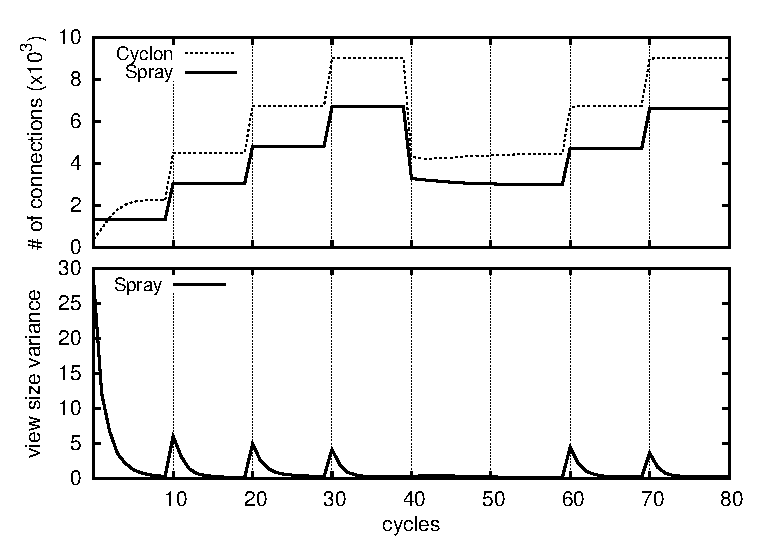
\includegraphics[width=0.47\textwidth]{img/spray/churn.eps}}
  \hspace{10pt}
  \subfloat[Figure B][\label{fig:churnB}The x-axis denotes the
  elapsed time in cycles. The y-axis denotes the average partial view size.]{
    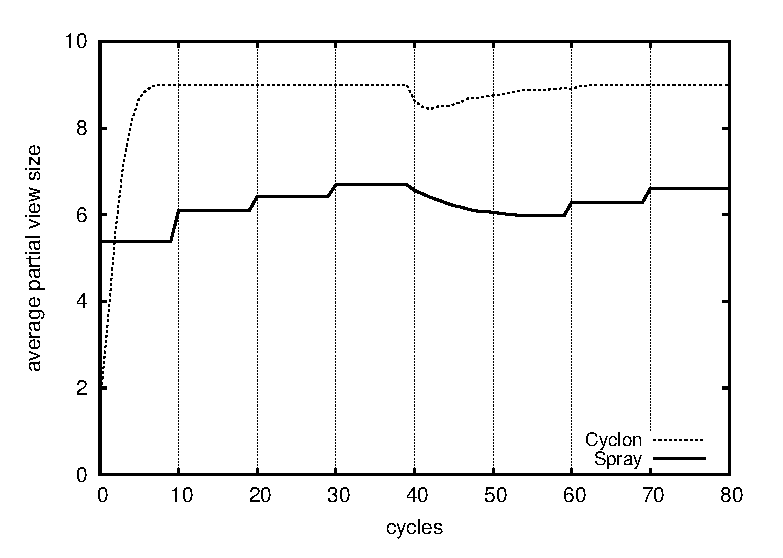
\includegraphics[width=0.47\textwidth]{img/spray/avgpv.eps}}
  \caption{\label{fig:churn}\CYCLON (partial view size configured to 9) and
    \SPRAY in a dynamic network. 2.5k peers join the network at cycles $0$,
    $10$, $20$, and $30$. Then 5k peers leave at cycle $40$. Finally 2.5k peers
    join at cycles $60$ and $70$. The final network contains 10k members.}
\end{figure*}

\begin{figure}
  \centering
  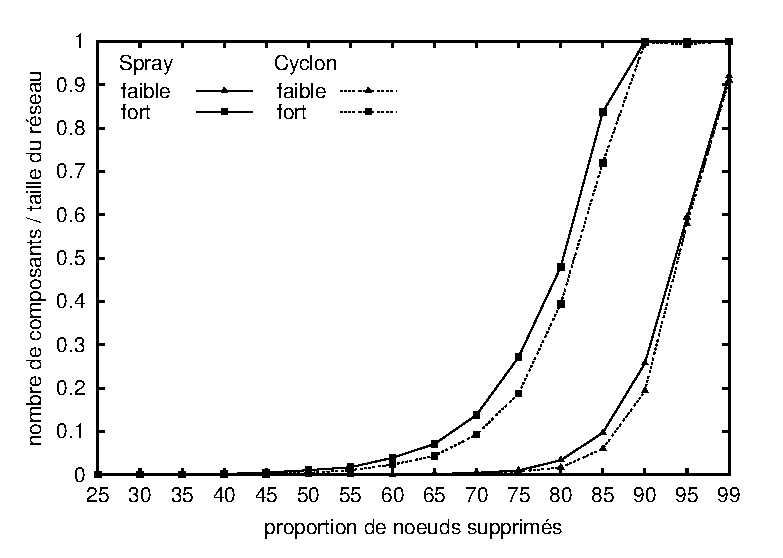
\includegraphics[width=\textwidth]{img/spray/resilience.eps}
  \caption{\label{fig:resilience}Robustness of \CYCLON and \SPRAY to massive
    failures. The x-axis denotes the percentage of peers removed at once in a
    network containing 10k members. The y-axis denotes the number of
    components over the current network size (after the removals). The
    measurements concern the weak and strong components which basically means
    the number clusters in undirected or directed graph respectively.}
\end{figure}


\begin{figure}
  \centering
  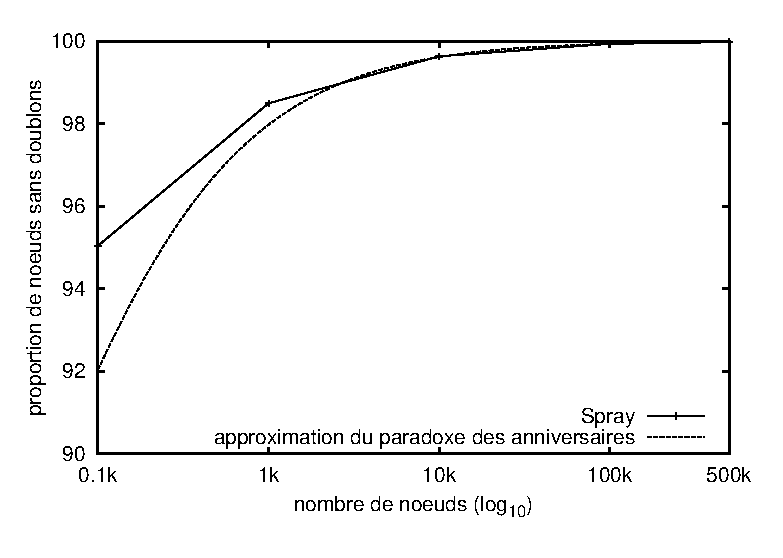
\includegraphics[width=\textwidth]{img/spray/duplicates.eps}
  \caption{\label{fig:duplicates}Duplicates in networks of different size: the
    $\log_{10}$-scaled x-axis denotes the network size while y-axis denotes the
    proportion of peers without any duplicates in their partial view.}
\end{figure}

\begin{figure}
  \centering 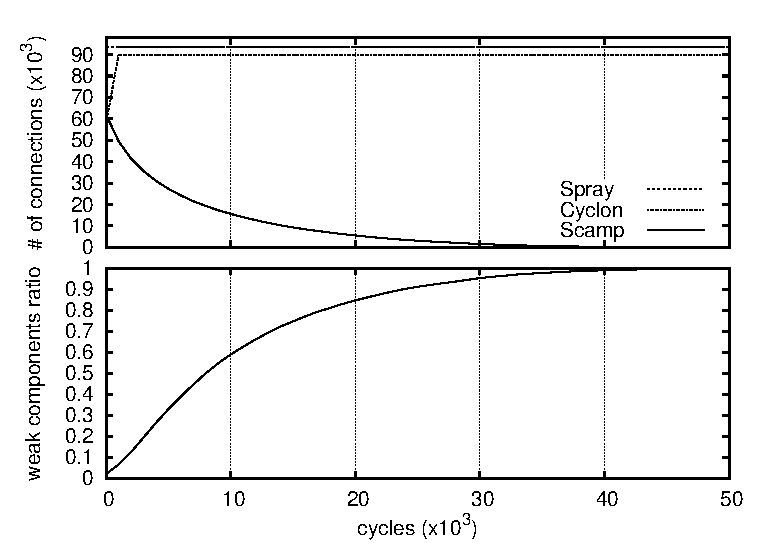
\includegraphics[width=\textwidth]{img/spray/degen.eps}
  \caption{\label{fig:degeneration}\CYCLON, \SCAMP, and \SPRAY in network
    subject to failures in the connection establishments. The x-axis denotes
    the elapsed time in cycles ($10^3$-scaled). The y-axis of the top figure
    denotes the global number of arcs ($10^3$-scaled). The y-axis of the bottom
    figure denotes the ratio of weak components over the current network size.}
\end{figure}

%%% Local Variables:
%%% mode: latex
%%% TeX-master: "../../paper"
%%% End:
